\section{Validating the Conjectures Empirically}
\label{sec:sim}

In this section, we evaluate our search heuristics for varying $U$ operator (i.e., varying values of $\theta$) and for $n = 2$ to $5$ and observe that they likely deliver
near-optimal initial state solutions to the \iso problem. 
Based on this observation, we show that our optimal solution Conjecture~\ref{conj:opt} is very
likely true as well the Conjecture~\ref{conj:avg}.
Our search heuristics implementation and 
experiment's raw data are open-source at\footnote{\url{https://github.com/caitaozhan/QuantumSensorNetwork}}.

% We utilize the Python-embedded modeling language CVXPY~\cite{diamond2016cvxpy} to implement the objective function $P()$ in Eqn.~\ref{eqn:objective}, the minimum probability of error incurred by using an optimal POVM in discriminating the final states.
% CVXPY uses the Splitting Conic Solver~\cite{sdp-solver} as the default SDP solver.


\begin{figure}
    \centering
    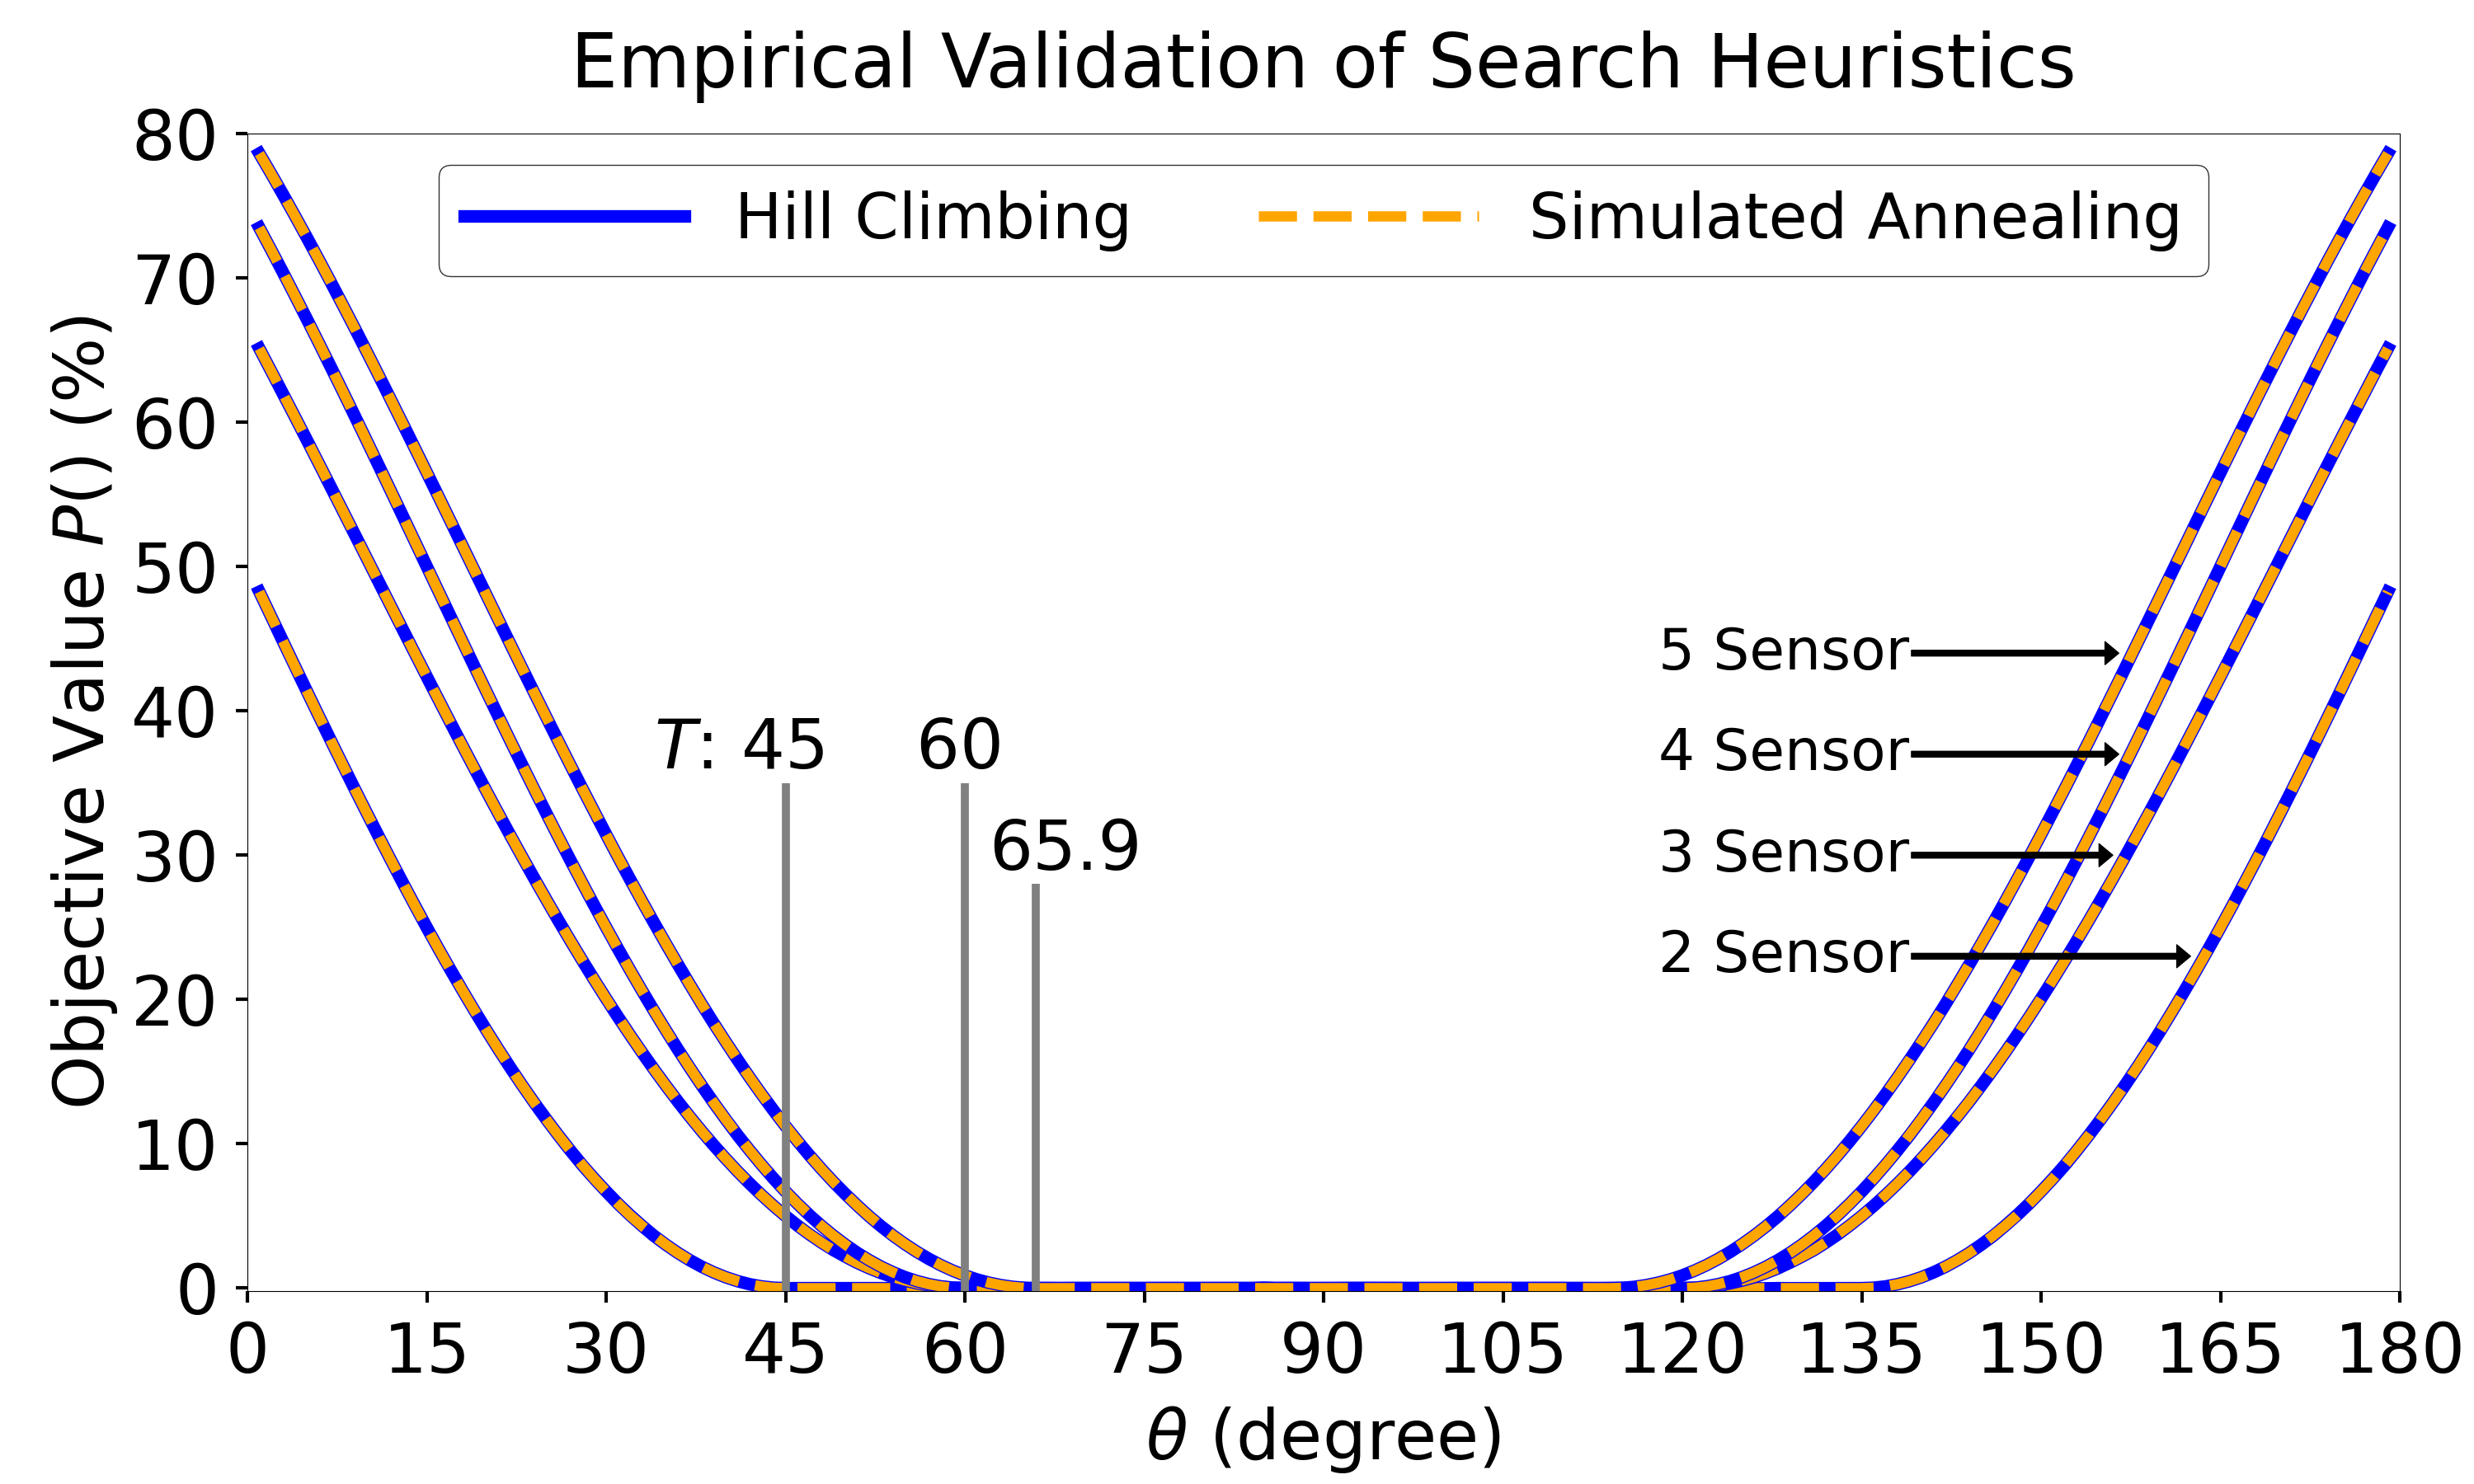
\includegraphics[width=0.75\textwidth]{chapters/tqc/figures/varying_theta_nsensors.png}
    \caption{Performance of the three search heuristics for varying $U$'s parameter $\theta$, for different number of sensors in the network. Genetic Algorithm (GA) is not shown explicitly, for clarity, but it also performs almost exactly the same as Hill-Climbing and Simulated Annealing (SA) which are plotted above.}
    \label{fig:heuristics}
\end{figure}


\para{Evaluation Setting.}
Recall that, without loss of generality, we assume the eigenvalues of 
$U$ to be $\{e^{+i\theta}, e^{-i\theta}\}$ with $U\ket{u_{\pm}}=e^{\pm i\theta}\ket{u_{\pm}}$ where $u_{\pm}$ are the
two eigenstates of $U$.
In our evaluations, we vary the $\theta$ in the range of $(0, 180)$ degrees, and
assume the prior probabilities of final states to be uniform. We consider four values of $n$, the number of sensors, viz., 2, 3, 4, and 5. Running simulations for much larger values of $n$ is infeasible due to the prohibitive computational resources needed. 
E.g., the estimated computation time to run any of the search 
heuristics for $n=10$ will take 10s of years, based on our 
preliminary 
estimates.\footnote{In our context, the Hill-Climbing heuristic goes through about 100
iterations and in each iteration, it needs to solve $4\cdot2^n$ instances of SDP formulations 
(Eqns~\ref{eqn:measure-sdp}-\ref{eqn:identity}) where $n$ is the number of sensors. 
%%%%%%%%%%%%
We use the Convex-Python CVXPY~\cite{diamond2016cvxpy} package
(which in turn used the Splitting Conic Solver~\cite{sdp-solver}) to solve our SDP formulations, and observe that it takes more than an hour to 
solve a single SDP instance for $n=10$; this suggests an estimate of 10s of years of computation time for $n=10$.}


\begin{figure}
    \centering
    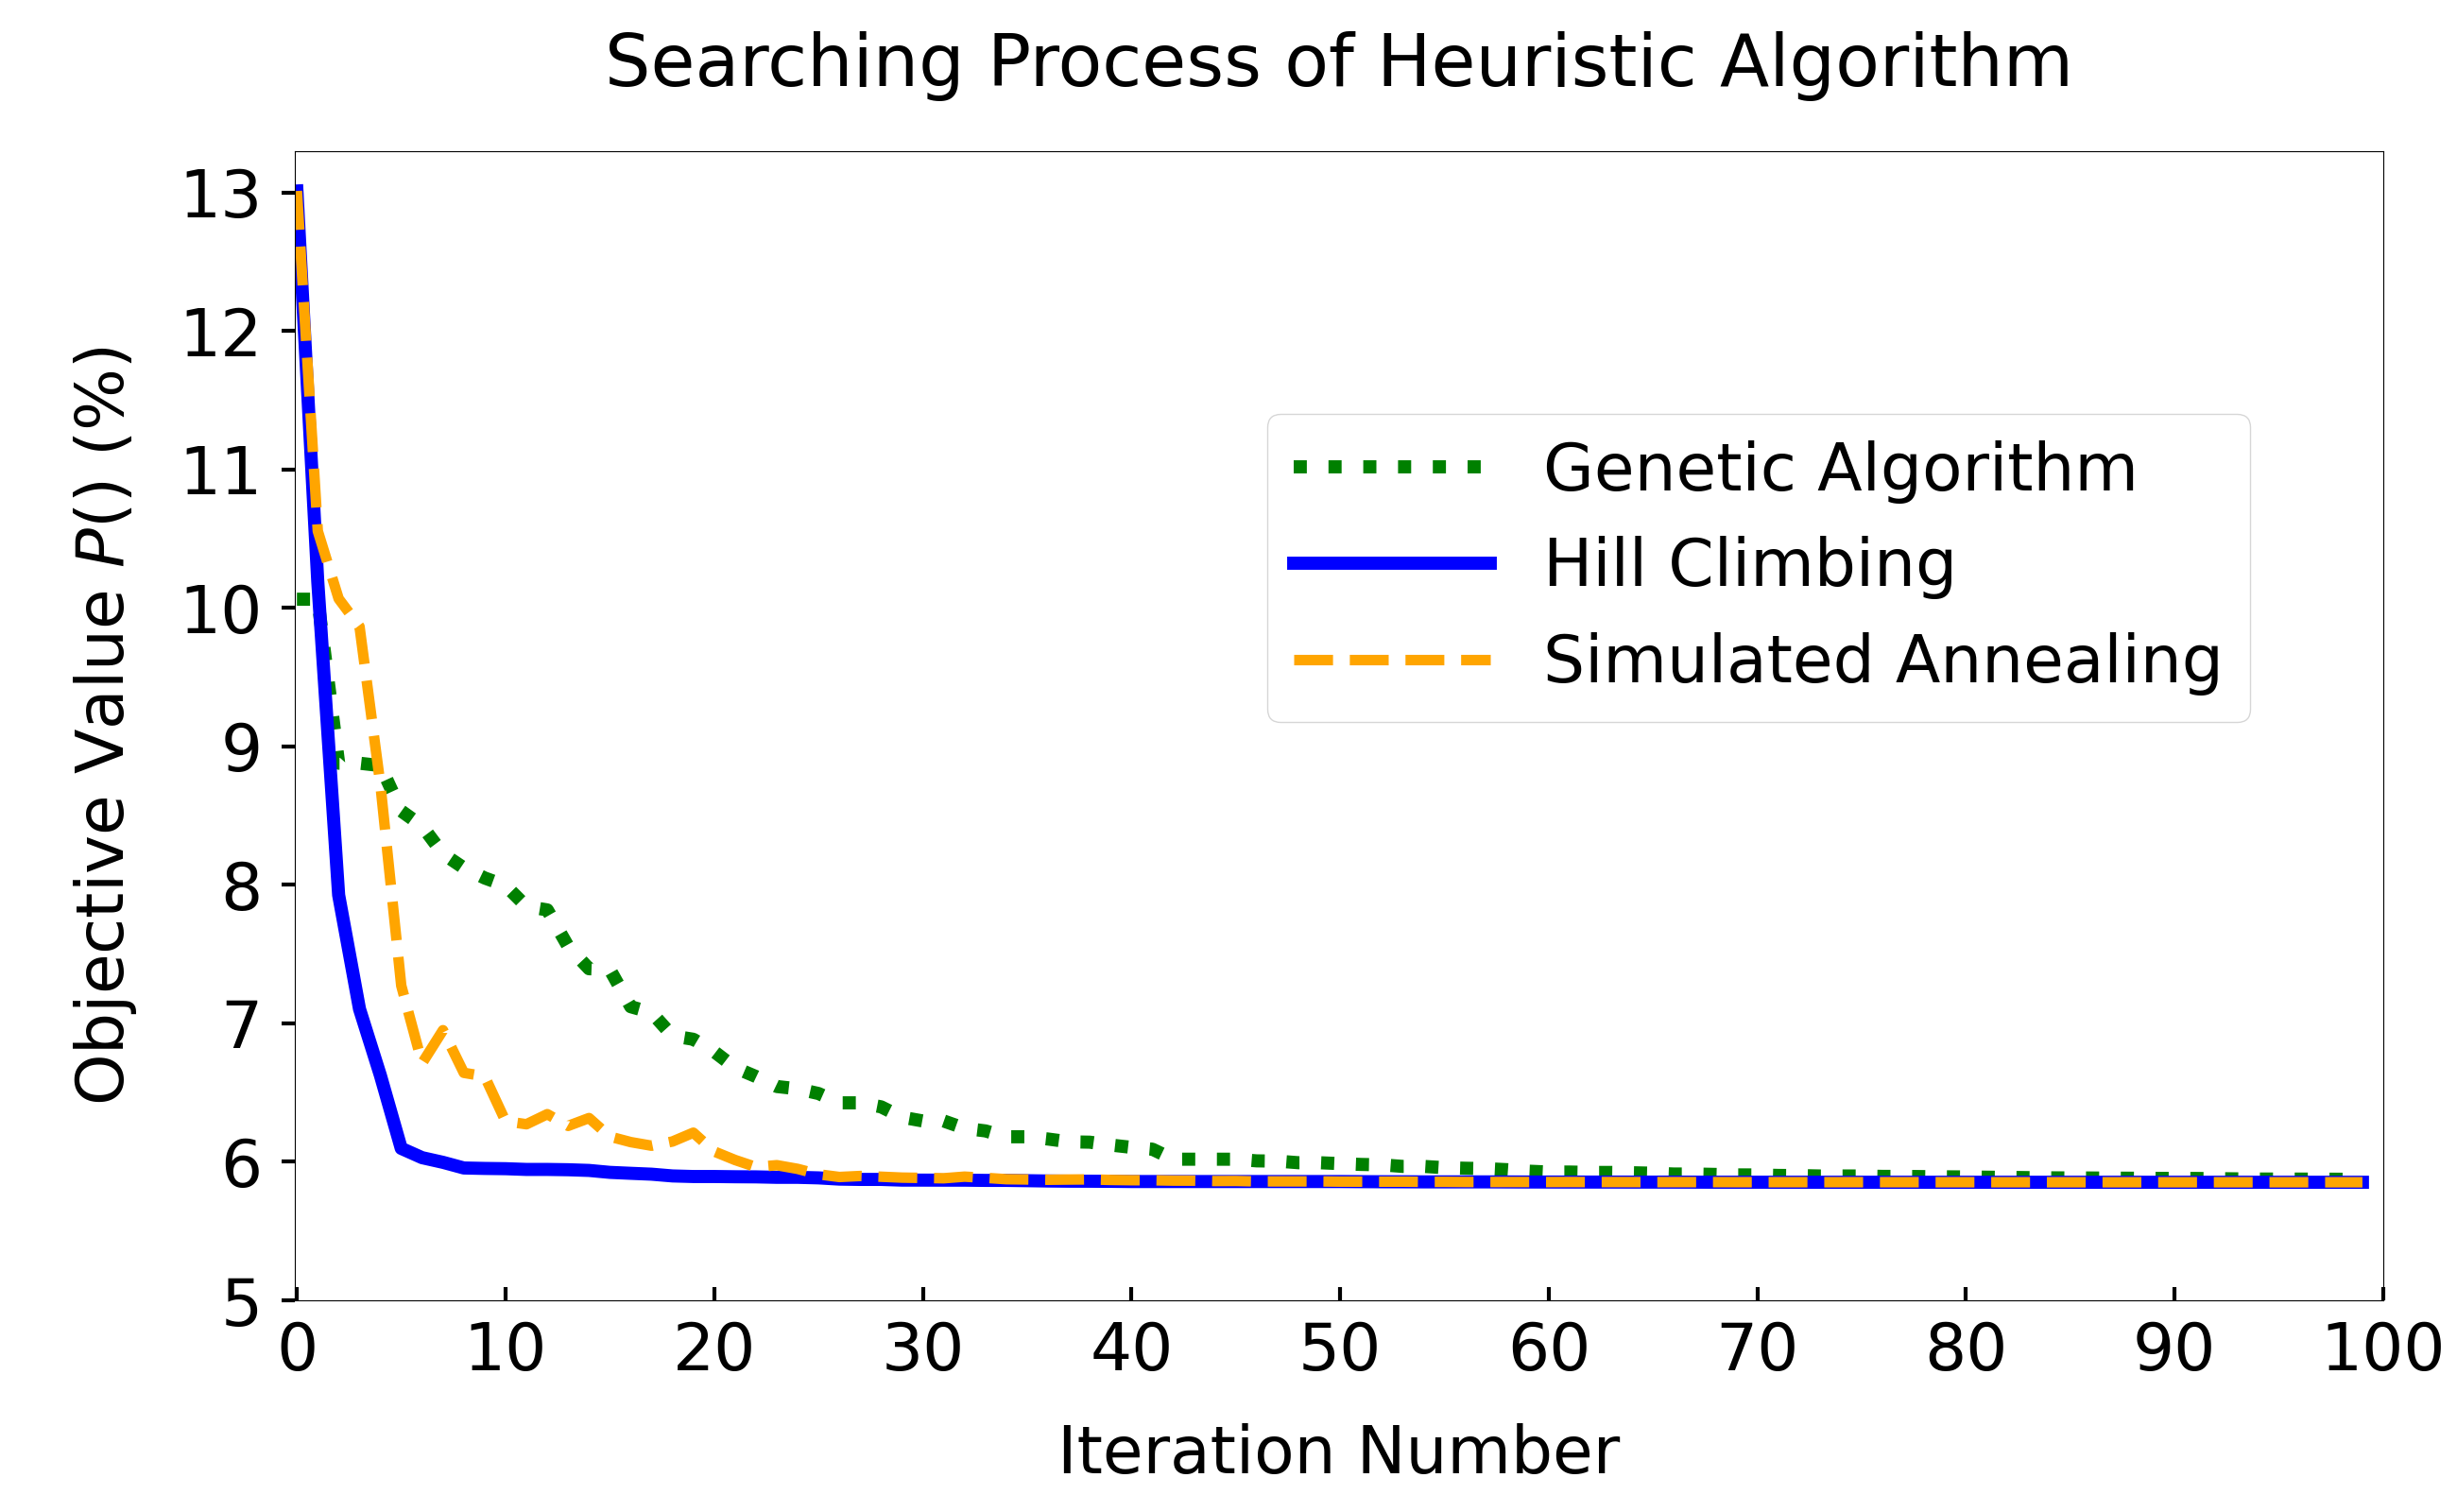
\includegraphics[width=0.75\textwidth]{chapters/tqc/figures/compare_methods_similar.png}
    \caption{The objective value $P()$, probability of error, of the candidate solution over iterations of the 
    three search heuristics for a special value of $\theta =46$ degrees and $n = 4$ sensors.}
    \label{fig:iterations}
\end{figure}

% estimates.\footnote{The time complexity of the Hill-Climbing algorithm can be estimated at $O(100.(4.2^n).f(n))$, 
% where 100 is the approximate number of iterations, $(4.2^n)$ is the number of SDP
% instances that arise in each iteration for $n$ number of sensors, and $f(n)$ is 
% the time complexity of an SDP instance in \S\ref{sec:searching} (Eqns~\ref{eqn:measure-sdp}-\ref{eqn:identity}). The SDP instances have $4^n$ variables, $n$ equations, and an input size of $O(n4^n)$. Lower bounding $f(n)$ by $o(n4^n)$, we get
% the lower-bound on the time complexity of the Hill-Climbing heuristic 
% as $o(400.n8^n)$. 
% We use the Splitting Conic Solver~\cite{sdp-solver} for solving our 
% SDP formulations as it is the default SDP solver in CVXPY.}


%(default in CVXPY).}





% The search heuristic algorithms are randomized algorithms (random initialization, generating random neighbors, etc), and the seed for the random number generator is 0 by default.

\para{Performance of Search Heuristics.}
% We first establish the credibility of the search heuristic algorithms Hill Climbing (HC), Simulated Annealing (SA), and Genetic Algorithm (GA). 
% If the heuristic algorithms are able to find an initial state such that the final states are mutually orthogonal when $\theta$ is in the range given by the Theorem~\ref{thm:nsensors}, then the heuristic algorithms are credible.
Fig.~\ref{fig:heuristics} shows the performance of the search heuristics
under varying $\theta$ and four values of $n = 2, 3, 4, 5$, in terms of the \iso objective function $P(\ket{\psi}, U)$ for the initial state solution $\ket{\psi}$. We make the following two observations:
\begin{enumerate}
    \item All three heuristics perform almost exactly the same.
    \item The heuristics deliver an initial state solution with $P(\ket{\psi}, U) = 0$ for the same range of $\theta$ given in Theorem~\ref{thm:nsensors}.
\end{enumerate}
We also observe that the heuristics perform the same for $\theta$ and $\pi - \theta$,
i.e., symmetric along the $\theta=\pi/2$ line. Thus, in the remaining plots, we only plot
results for $\theta \in (0, \pi/2]$.
%%%%%%%%%%%%%%%%%%%%%%
Fig.~\ref{fig:iterations} shows the convergence rates of the three heuristics for a specific value of $\theta=46$ degrees and $n=4$ sensors. 
We observe that HC converges the fastest, followed by SA and GA.
After 100 iterations, the HC and SA end at a probability of error of $5.85\%$, while GA ends at $5.86\%$.



\begin{figure}[ht]
    \centering
    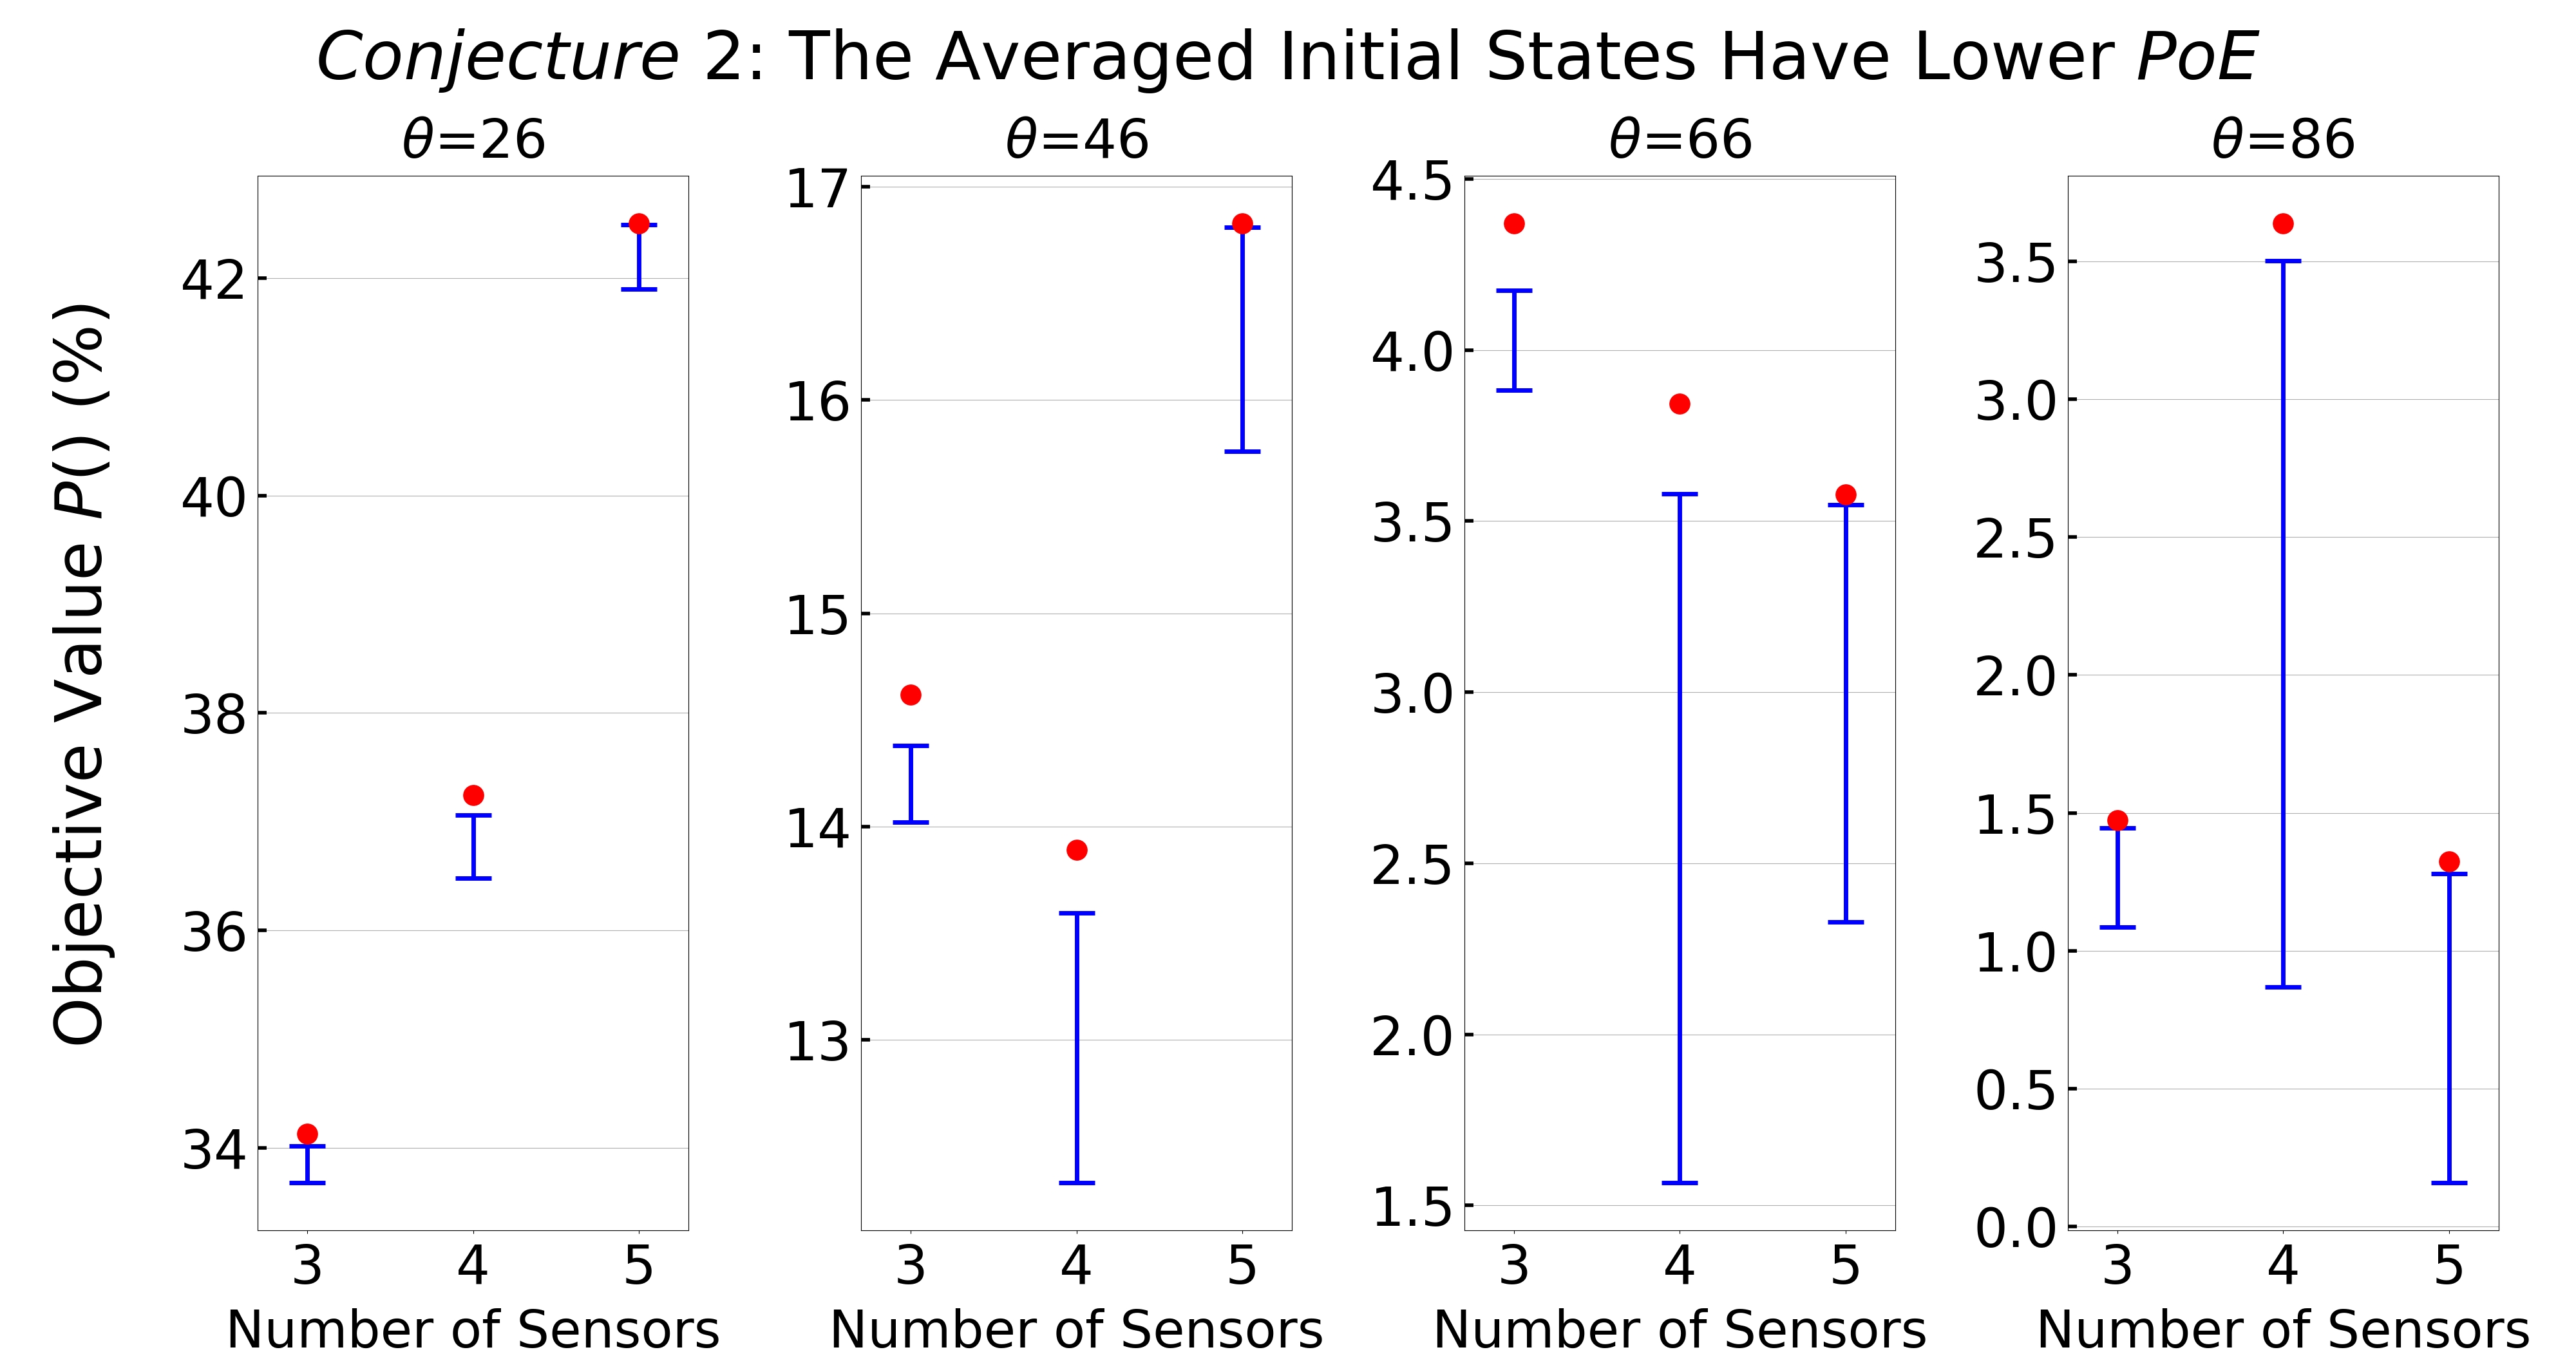
\includegraphics[width=0.8\textwidth]{chapters/tqc/figures/lemma2.png}
    \caption{Empirical validation of Conjecture~\ref{conj:avg}. For four different values of $\theta$ and three different values of $n$, we show that
    the objective value (Probability of Error) of the original initial state (the red circle) remains higher than the objective value of the many ``averaged'' states (range shown by blue the bar).}
    \label{fig:lemma2}
\end{figure}



\para{Empirical Validation of Conjecture~\ref{conj:avg}.}
Recall that Conjecture~\ref{conj:avg} states that an ``average'' solution 
of two \iso solutions with
equal objective values have a lower objective value. To empirically validate
Conjecture~\ref{conj:avg}, we generate a random state $\ket{\psi}$, and then, 
generate  $n!-1$ additional states of the same objective value $P()$ by 
renumbering the sensors as discussed in Theorem~\ref{thm:final}'s proof. 
Then, we take many pairs of these states, average them, and compute the
objective value. 
%%%%%%%%%%%%%%%%%%%%%%%
Fig.~\ref{fig:lemma2} plots the objective value of the original state $\ket{\psi}$,
and the range of the objective values of the averaged states. We observe that the
objective values of the averaged states are invariably less than that of 
$\ket{\psi}$. 

\begin{figure}[ht]
    \centering
    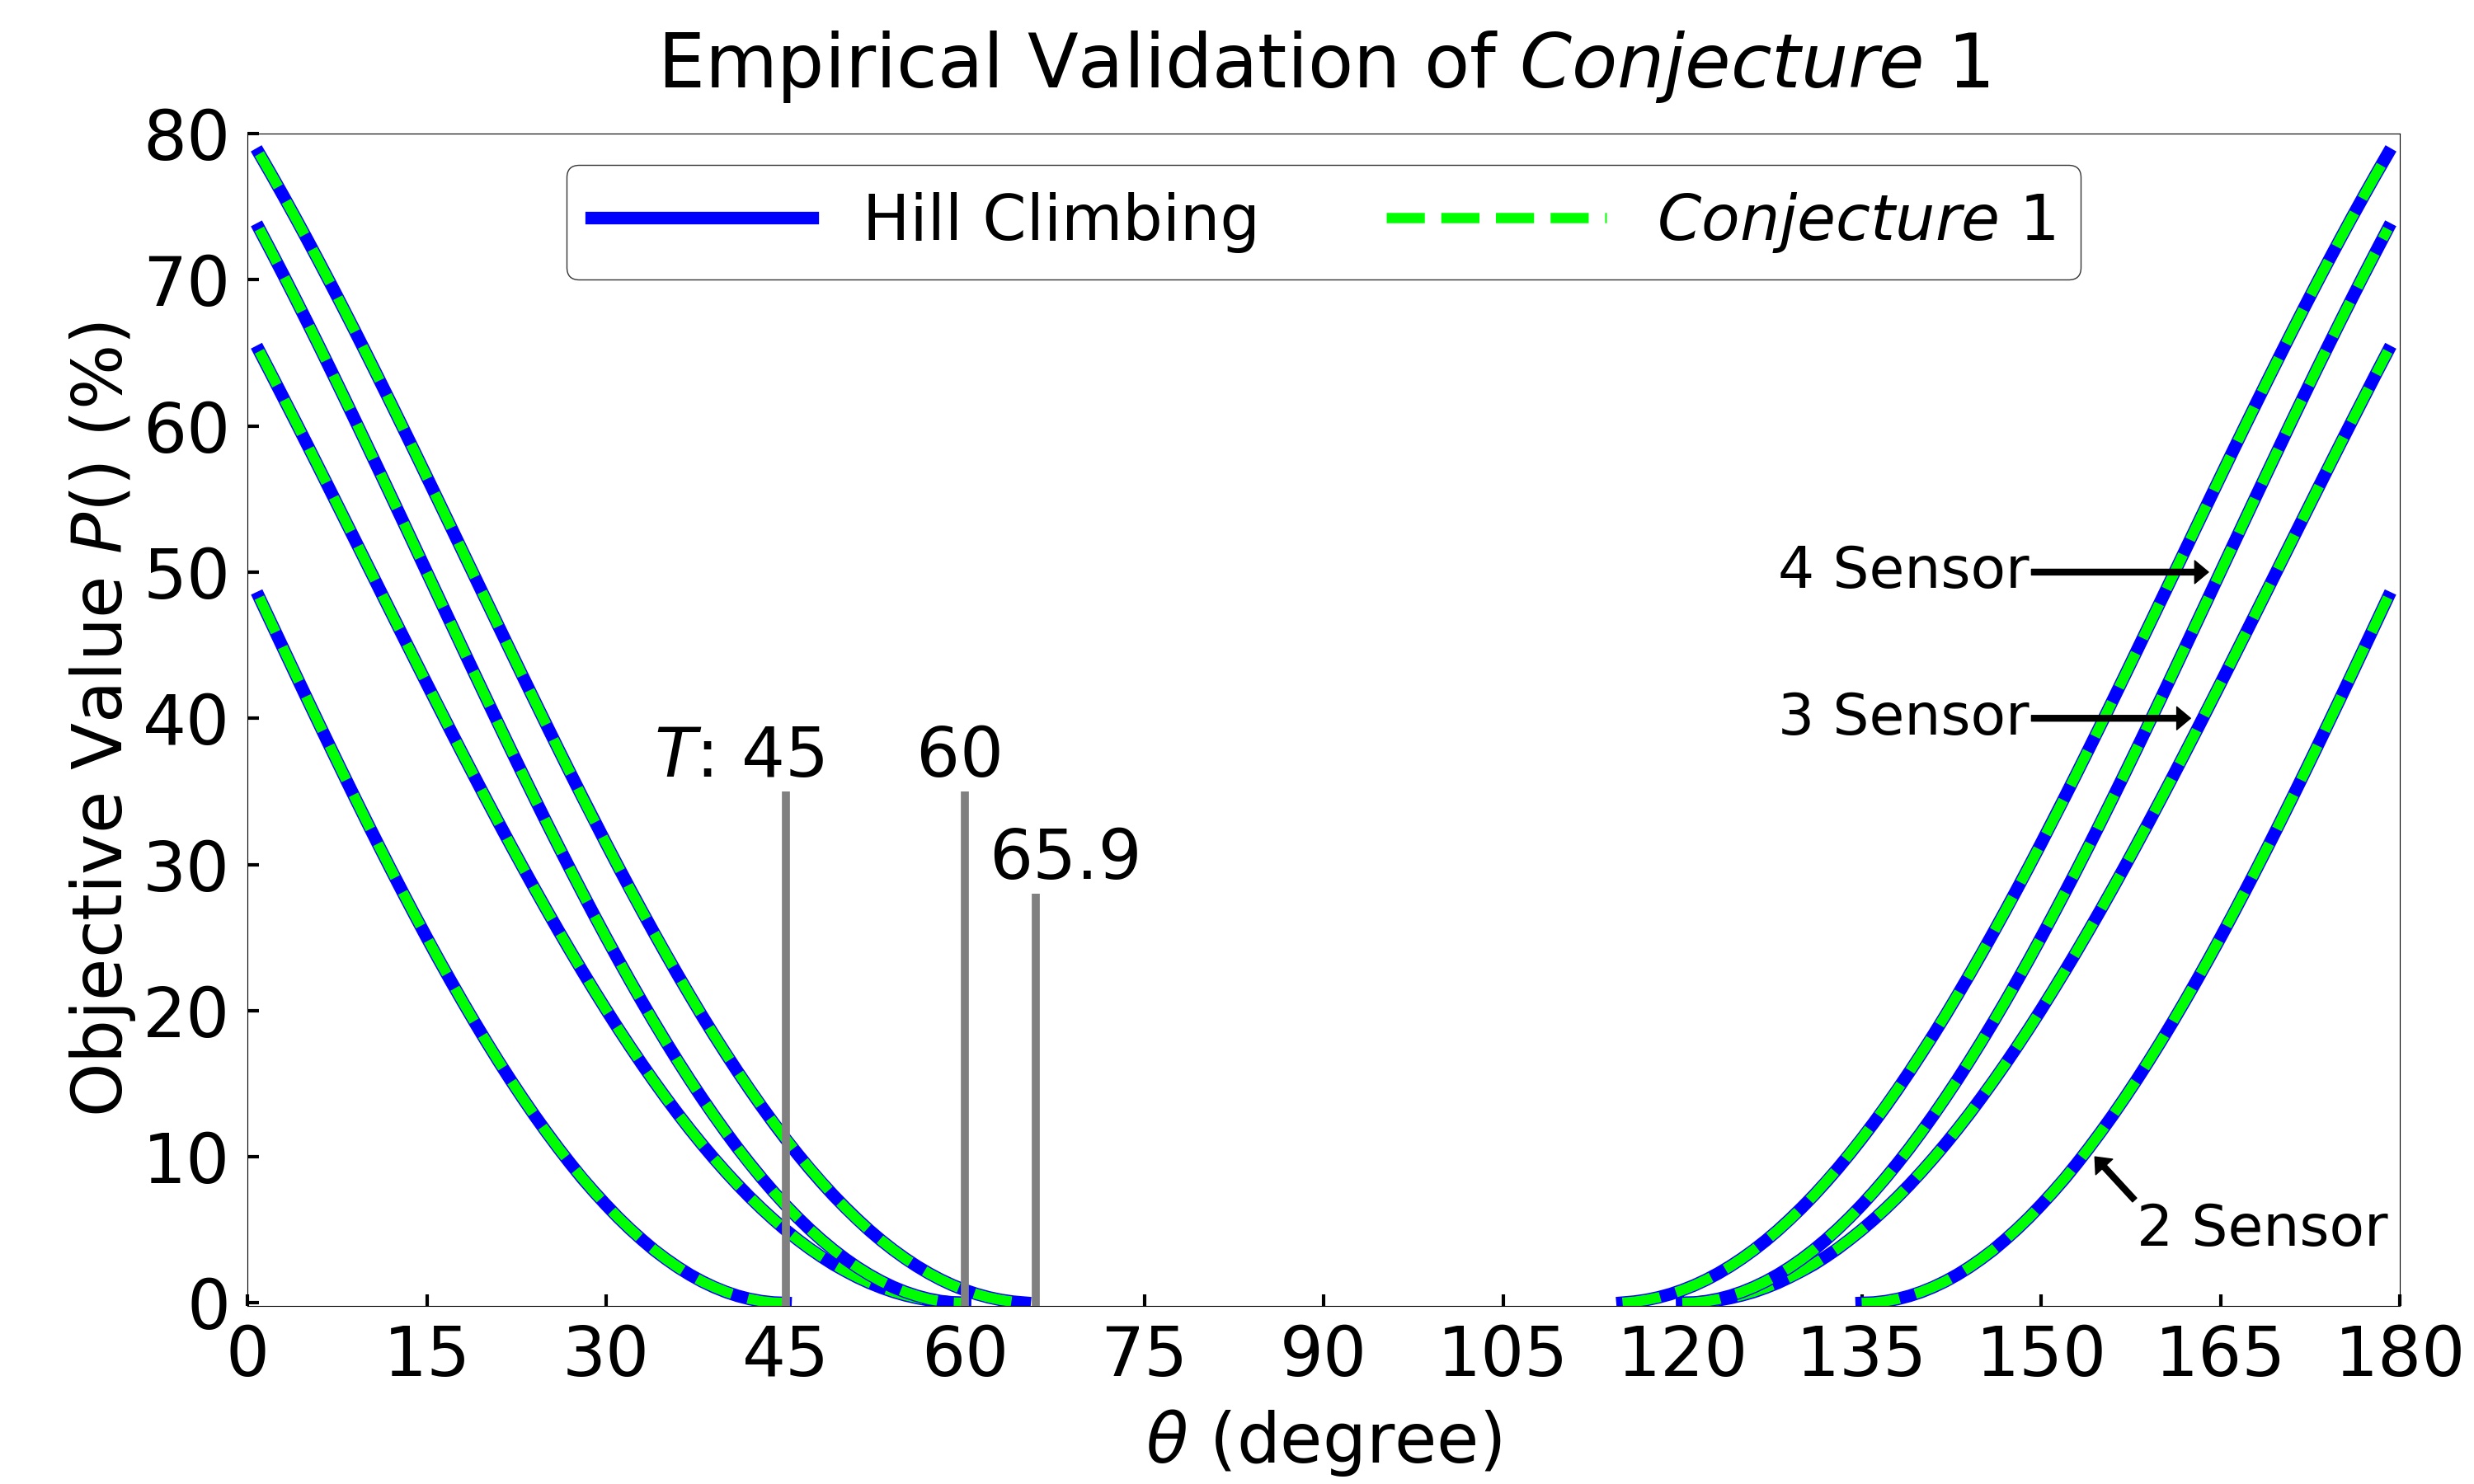
\includegraphics[width=0.75\textwidth]{chapters/tqc/figures/conjecture.png}
    \caption{The Conjecture~\ref{conj:opt}'s solution performs almost exactly as the Hill-Climbing heuristic when $\theta \in (0, T] \cup [180-T, 180),$ degrees, where $T$ is from Theorem~\ref{thm:nsensors}. 
    For $n=2$, Conjecture~\ref{conj:opt}'s solution matches with the provably optimal solution from~\cite{Hillery_2023} with $T$ being 45 degrees.}
    \label{fig:conjecture}
\end{figure}

% \para{Empirical Validation of Conjecture~\ref{lema:angle}.}
% Recall that Conjecture~\ref{lema:angle} states that the probability of error in discriminating a set of ``symmetric'' final states increases with the decrease in the
% common pairwise-angle (or, equivalently, increase in the pairwise inner-product value) between them.
% To empirically validate Conjecture~\ref{lema:angle}, we generate final states with equal
% pairwise inner-products using an iterative process as follows. 
% We start with a $n$-dimension state vector $\phi_1 = [1, 0, \cdots, 0]$, and
% in the  $i^{th}$ iteration, we generate the state $\phi_i$ of the type
% $\phi_i = [a_{i0}, a_{i1}, \cdots, a_{ii}, 0, 0,  \cdots, 0]$.
% %%%%%%%%%%%%%%%%%%%%
% To create $\phi_i$, we set $a_{ij} = a_{i-1, j}$ for all $0 \leq j \leq i-2$, and then
% (i) set $a_{i, i-1}$ to ensure that $\bra{\phi_{i-1}}\ket{\phi_{i}}$ equal to the common
% inner-product value, and (ii) 
% set $a_{ii}$ to ensure $\bra{\phi_{i}}\ket{\phi_{i}} = 1$. 
% %%%%%%%%%%%%%%%%%%%%%%%%%
% Fig.~\ref{fig:lemma3} shows the probability of error (obtained by solving the SDP formulations) in discriminating a set of states created as above, for different 
% $n$, and varying values of $x$, the common inner-product value. We observe
% that the probability of error monotonically increases with increases in $x$.



% \begin{figure}
%     \centering
%     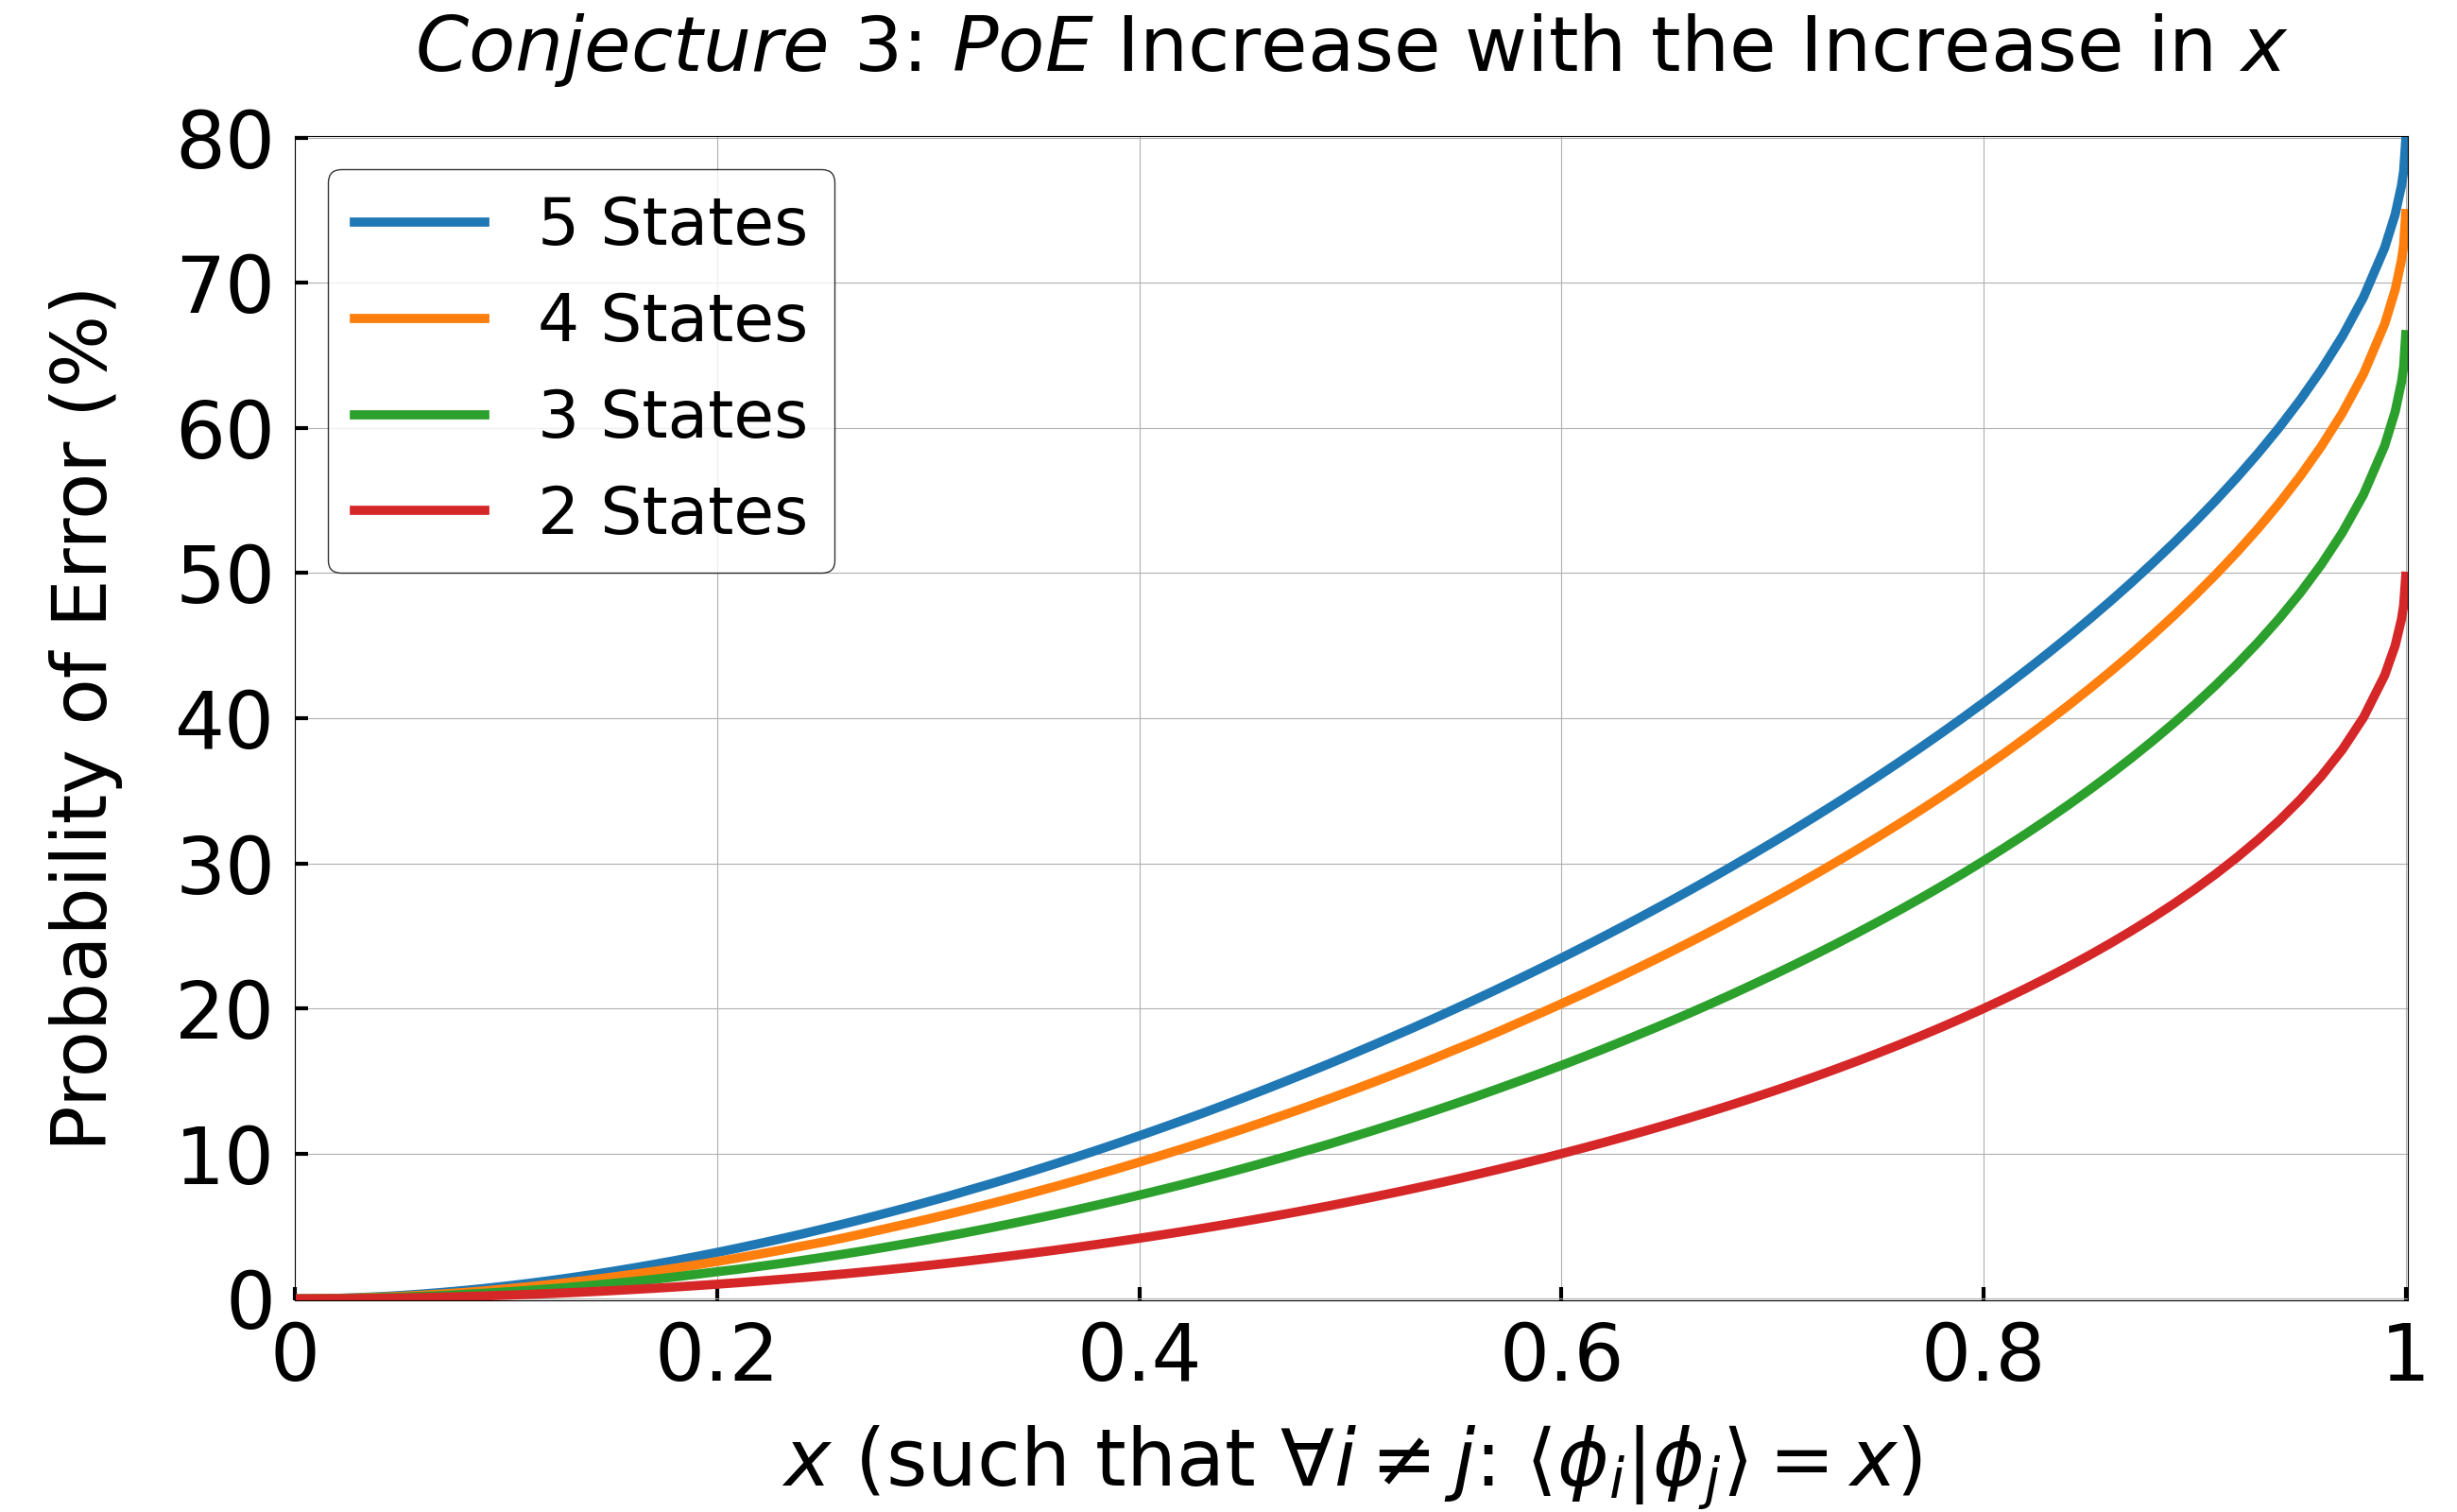
\includegraphics[width=0.44\textwidth]{figures/lemma3.png}
%     \caption{Empirical validation of Conjecture~\ref{lema:angle}. For different number of (final) states, we see that the probability of error in discriminating the created ``symmetric'' (final) states increases with the increase in the common pairwise inner-product value.}
%     \label{fig:lemma3}
% \end{figure}

\para{Empirical Validation of the Optimal Solution Conjecture~\ref{conj:opt}.}
We now evaluate the performance of the initial state solution obtained by Conjecture~\ref{conj:opt} and compare it with the solution delivered by 
one of the search heuristics--Hill Climbing (HC).
Here, we consider $\theta \in (0, T) \cup (180-T, 180)$ degree, where $T$ is 
as defined in Theorem~\ref{thm:nsensors}.
In Fig.~\ref{fig:conjecture}, we observe that the HC heuristic and Conjecture~\ref{conj:opt} solutions have identical performance, suggesting that
Conjecture~\ref{conj:opt}'s solution is likely optimal based on our earlier observation
that the search heuristics likely deliver optimal solutions.



% \begin{figure}
%     \centering
%     \includegraphics[width=0.6\textwidth]{figures/symmetry_varymethod.png}
%     \caption{Symmetry-index of the candidate solutions over iterations of the three search heuristics for $\theta = $ 46 degrees. }
%     \label{fig:symmetry-methods}
% \end{figure}

% \begin{figure}
%     \centering
%     \includegraphics[width=0.6\textwidth]{figures/symmetry_varytheta.png}
%     \caption{Symmetry-index of the candidate solutions over iterations of the HC heuristic for different values of $\theta$.}
%     \label{fig:symmetry-theta}
% \end{figure}

\begin{figure}
    \centering
    \begin{subfigure}[t]{0.49\textwidth}
	\includegraphics[width=\textwidth]{chapters/tqc/figures/symmetry_varymethod.png}
	\caption{The three search heuristics for $\theta = $ 46 degrees. }
        \label{fig:symmetry-methods}
    \end{subfigure}
    \qquad
    \hspace{-0.3in}
    \begin{subfigure}[t]{0.49\textwidth}
	\includegraphics[width=\textwidth]{chapters/tqc/figures/symmetry_varytheta.png}
	\caption{The HC heuristic for different values of $\theta$.}
        \label{fig:symmetry-theta}
    \end{subfigure}
    \caption{Symmetry-index of the candidate solutions over iterations.}
    \label{fig:symmetry-iteration}
\end{figure}

\begin{figure}
    \centering
    \begin{subfigure}[t]{0.49\textwidth}
	\includegraphics[width=\textwidth]{chapters/tqc/figures/poe_symmetry.png}
	\caption{Probability of Error vs.\ Symmetry Index}
        \label{fig:poe_symmetry}
    \end{subfigure}
    \qquad
    \hspace{-0.3in}
    \begin{subfigure}[t]{0.49\textwidth}
	\includegraphics[width=\textwidth]{chapters/tqc/figures/poe_symmetry_zoomin.png}
	\caption{Probability of Error vs.\ Symmetry Index, zoomed-in for low values of symmetry index}
        \label{fig:poe_symmetry_zoom}
    \end{subfigure}
    \caption{The correlation between the objective value (probability of error) and the symmetry index.}
\end{figure}

\para{Symmetry ``Index'' vs.\ Objective Value (Probability of Error).}
In this final experiment, we investigate the impact of the symmetry of coefficients on the objective value of an initial state. 
Here, we only do experiments for $n=3$ number of sensors.
To this end, we define a notion of {\em symmetry index} which quantifies the symmetry of coefficients in a given initial
state. In particular, we define the {\em symmetry index} for an initial state
$\ket{\psi} = \sum\limits_j \psi_j \ket{j}$ as:  
\begin{equation}
\sum_{k=0}^{n} \sum_{|\psi_i|^2, |\psi_j|^2 \in S_k} (|\psi_i|^2 - |\psi_j|^2)^2
\label{eqn:symmety} 
\end{equation}
\noindent
where $S_k$ is the $k$th symmetric set as defined in Theorem~\ref{thm:nsensors}.
The symmetric index being zero implies that within each symmetric set, all the coefficient-squares are equal.
%%%%%%%%%%%%%%%%%%%%%%%%%%%%%%
Fig.~\ref{fig:symmetry-iteration} shows that the search heuristic essentially generates solutions with lower and lower symmetry index, and finally, converges to a solution with zero symmetry index value. 
This is true for all three search heuristics (Figs.~\ref{fig:symmetry-methods}) and for varying $\theta$ (Fig.~\ref{fig:symmetry-theta}).
Given Fig.~\ref{fig:iterations} already shows that the objective value decreases as the searching iterations go on, we can conclude that the objective value and the symmetry index decrease simultaneously when the iterations go on.
Furthermore in Fig.~\ref{fig:poe_symmetry}, we show the correlation between symmetry index and objective value through a scatter plot---with the objective value generally decreasing with the decrease in symmetry index. 
Fig.~\ref{fig:poe_symmetry_zoom} zooms in to the later iterations of the heuristics wherein the symmetry index is very low (less than 0.08) to show a clearer view of the correlation.

% \begin{figure}
%     \centering
%     \includegraphics[width=0.6\textwidth]{figures/poe_symmetry.png}
%     \caption{Probability of Error vs.\ Symmetry Index}
%     \label{fig:poe_symmetry}
% \end{figure}


% \begin{figure}
%     \centering
%     \includegraphics[width=0.6\textwidth]{figures/poe_symmetry_zoomin.png}
%     \caption{Probability of Error vs.\ Symmetry Index, for low values of symmetry index}
%     \label{fig:poe_symmetry_zoom}
% \end{figure}


